\documentclass[12pt]{beamer}

\usepackage{beamerthemesplit}


\usepackage{beamerthemesplit}

\usepackage{beamerStatisticsTAMU} 

\logo{\includegraphics[height=1.5cm]{STAT_Horz-Aggie-Maroon.pdf}\vspace{220pt}}


\usepackage{amsmath}
\usepackage{amssymb}
\usepackage{verbatim}
\usepackage{bibentry}
%\usepackage{biblatex}
%\usepackage{natbib}
\newcommand{\argmin}[1]{\underset{#1}{\operatorname{argmin}}\text{ }}
\newcommand{\argmax}[1]{\underset{#1}{\operatorname{argmax}}\text{ }}
\usepackage{bbm}
\usepackage{bm}
\usepackage[absolute,overlay]{textpos}

\newcommand{\Var}{\text{Var }}
\newcommand{\Cov}{\text{Cov }}
\newcommand{\E}{\mathbb{E}}
\newcommand{\V}[1]{{\bm{\mathbf{\MakeLowercase{#1}}}}} % vector
\newcommand{\M}[1]{{\bm{\mathbf{\MakeUppercase{#1}}}}} % matrix
\newcommand{\todo}[1]{{\color{red}TODO: #1}}

\newcommand{\w}{0.8in}
\newcommand{\h}{1in}
\usepackage{graphicx}
\newcommand{\indep}{\rotatebox[origin=c]{90}{$\models$}}

\newtheorem{assumptions}{Assumptions}

\setbeamertemplate{headline}[default]
\setbeamertemplate{footline}[page number]
\setbeamertemplate{navigation symbols}{}
\setbeamertemplate{bibliography item}[text]

\title{Parsimonious Models for Functional Data: Discovering and Characterizing RR Lyrae from Sparsely Sampled Light Curves}
\author{James Long}
%%\institute{UC Berkeley}
\date{\today}
\begin{document}

\frame{\titlepage}

\frame{\tableofcontents}

\AtBeginSection[]
{
  \begin{frame}<beamer>
    \frametitle{Outline}
    \tableofcontents[currentsection,currentsubsection]
  \end{frame}
}


%%%%%%%%
%%%%%%%% TODO: redo first section with more emphasis on multiband, lomb scargle
%%%%%%%%


\section{Time Domain Astronomy and Variable Stars}

\begin{frame}{Periodic Variable Stars}
\textbf{Periodic variables:} Stars that repeat brightness variation over a fixed period.
\begin{center}
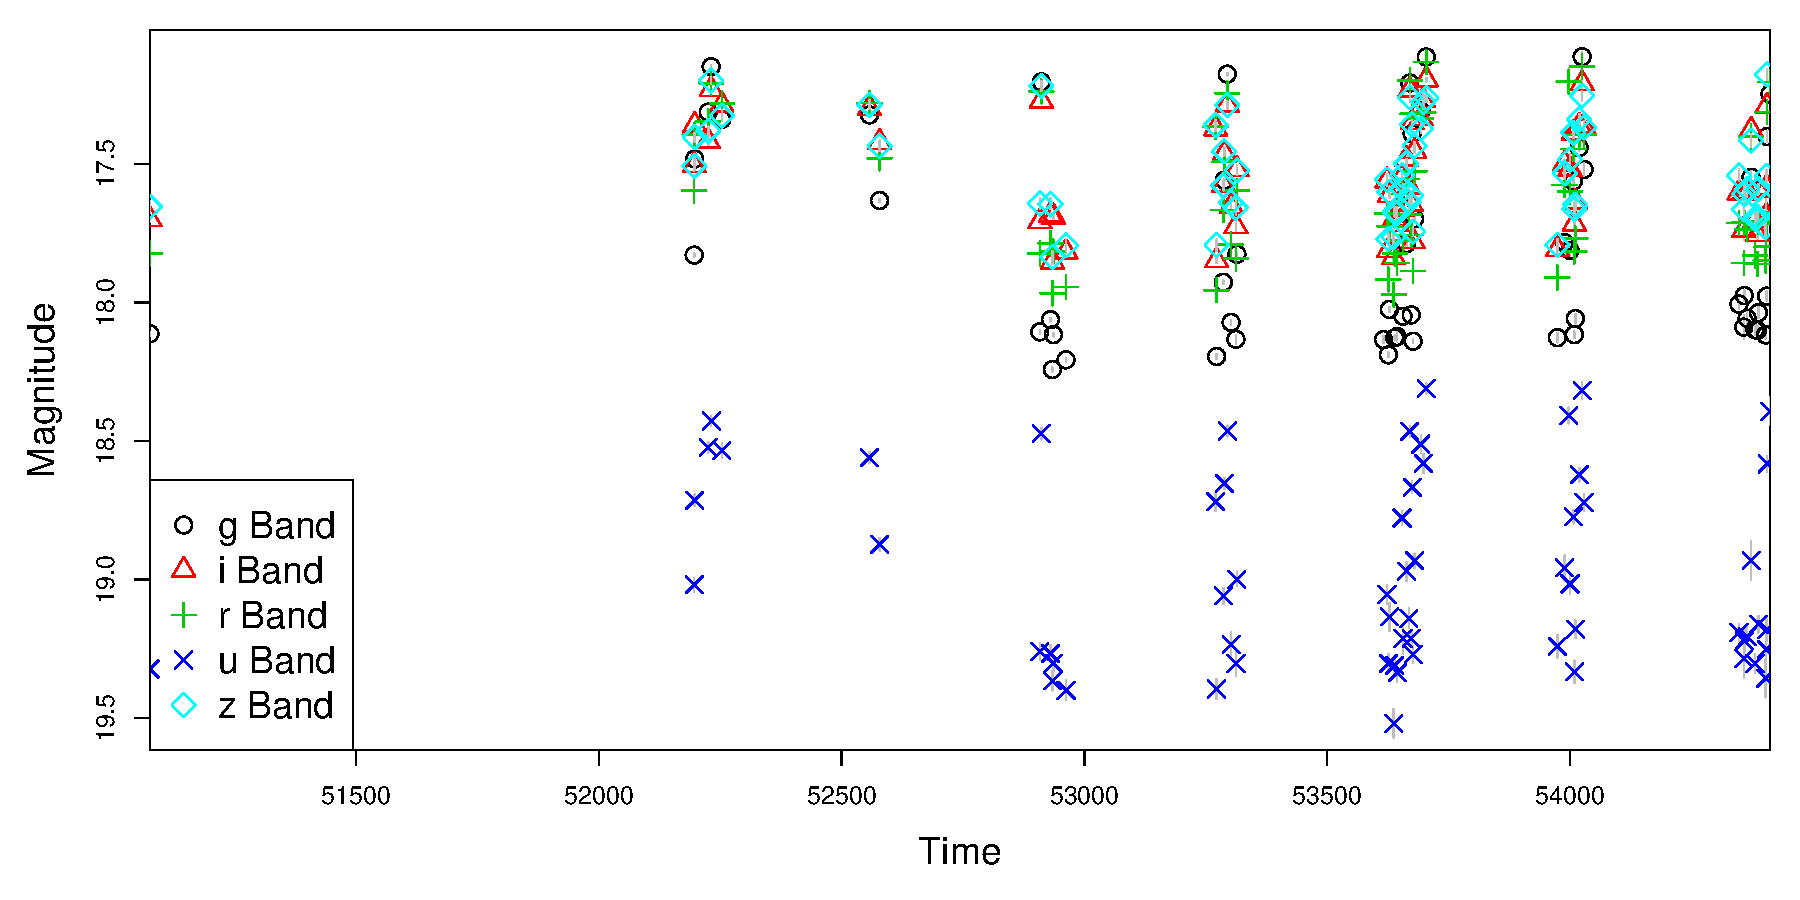
\includegraphics[scale=.3]{figs/unfolded_13350.pdf}
\end{center}
\begin{itemize}
\item Star observed $\approx 250$ times in $5$ bands, $u,g,r,i,z$.
\item Data for star is $D=\{t_{jb},m_{jb},\sigma_{jb}\}_{j=1}^{n_b}$ for $b=1,\ldots,B$.
\item Observe brightness $m_{jb}$ at time $t_{jb}$ with uncertainty $\sigma_{jb}$ in band $b$.
\end{itemize}
\end{frame}


\begin{frame}{Folded Light Curve of Periodic Variable}
\textbf{Folded light curve:} Brightness versus time modulo period.
\begin{center}
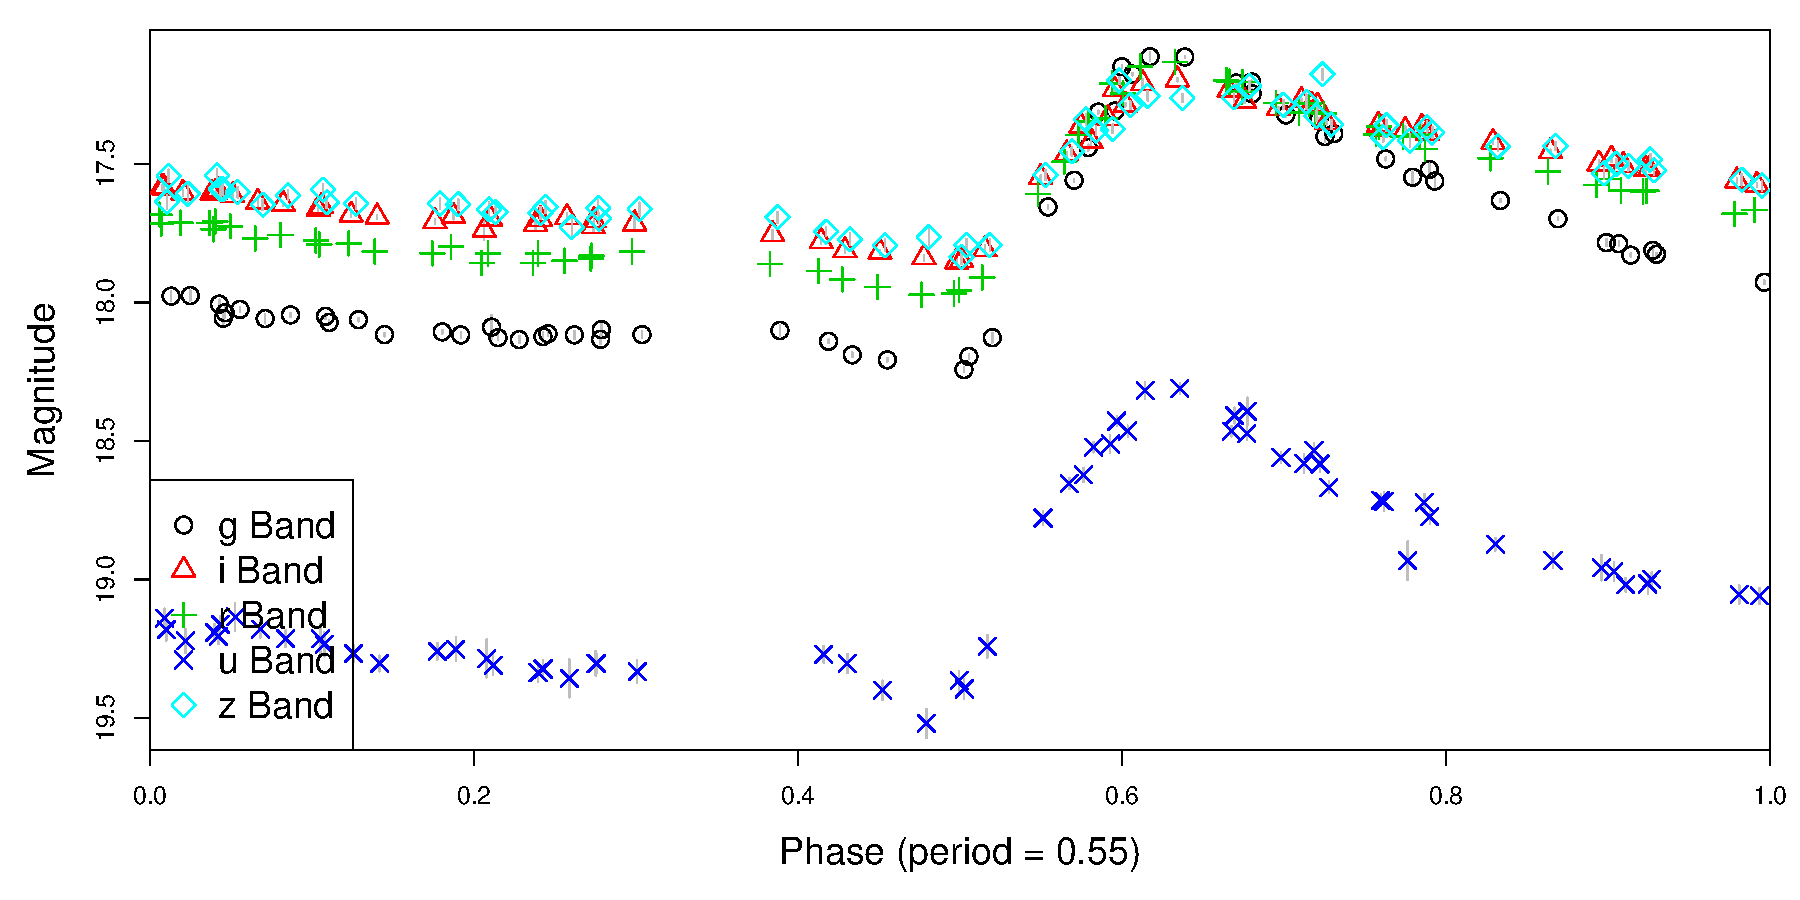
\includegraphics[scale=.3]{figs/folded_13350.pdf}
\end{center}
\end{frame}


\begin{frame}{SDSS--III Stripe 82 \cite{ivezic2007sloan}}
\begin{itemize}
\item Collected $\approx 60,000$ variables in Stripe 82 Region
\item Variables belong to different \textbf{classes}
\item Some periodic, some not
\end{itemize}


\underline{Two Examples}

\vspace{-.2in}

\begin{center}
Eclipsing Binary\\
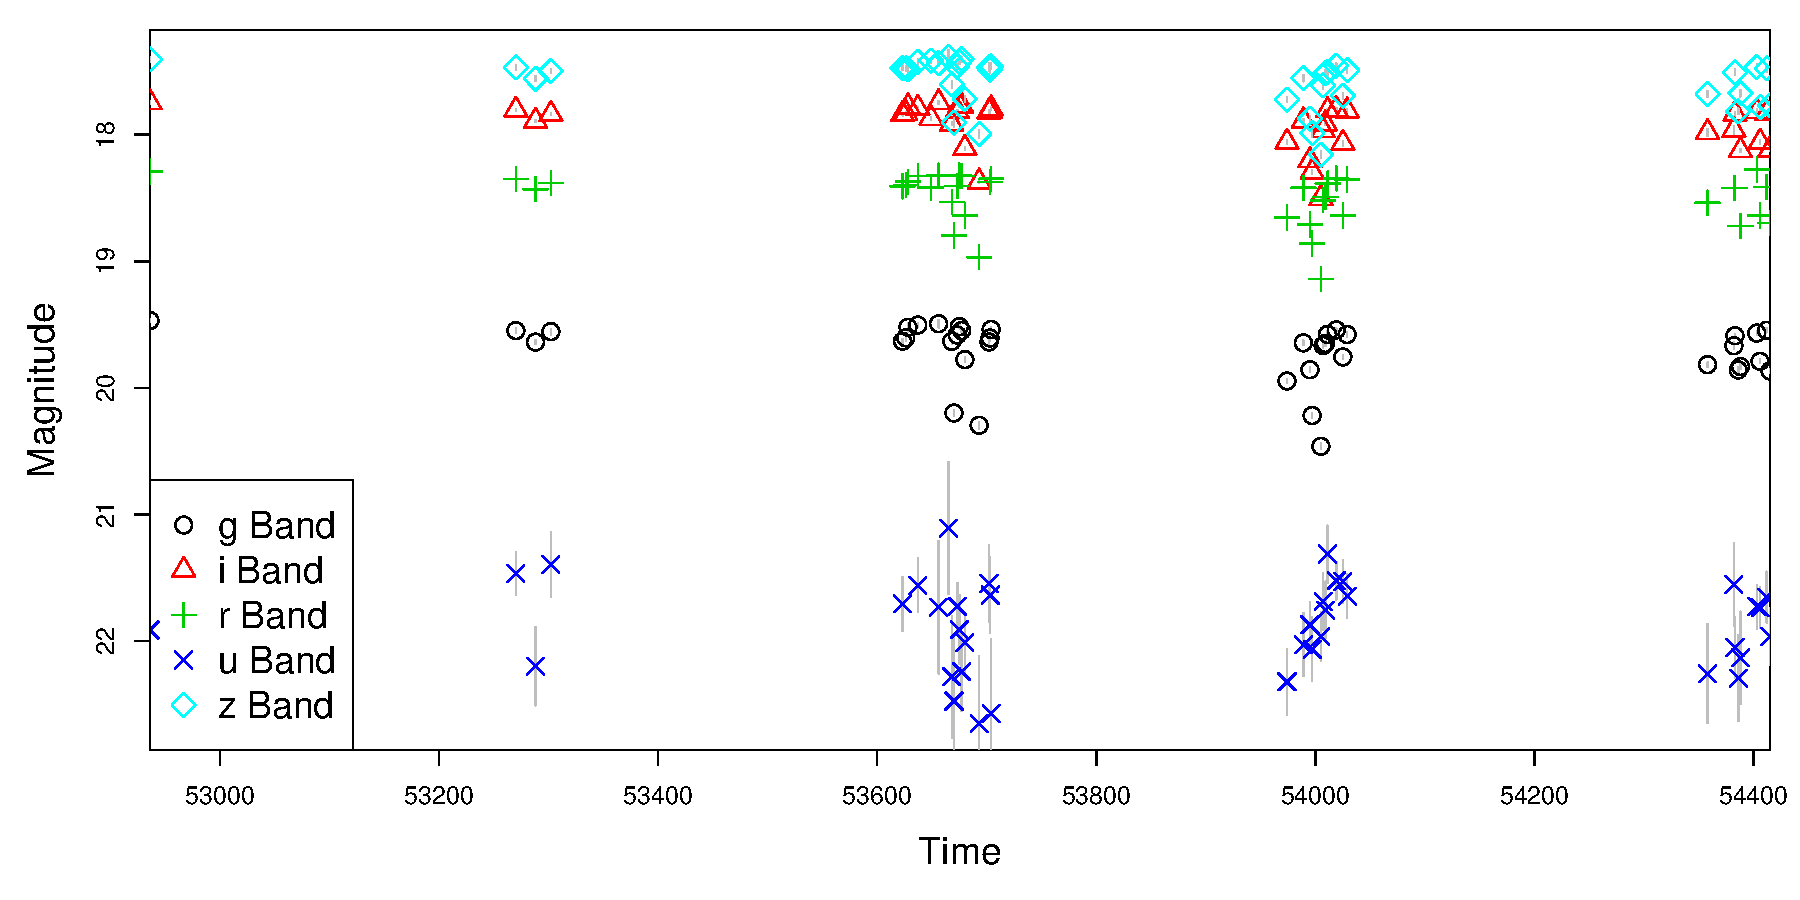
\includegraphics[scale=.15]{figs/unfolded_4183016.pdf}
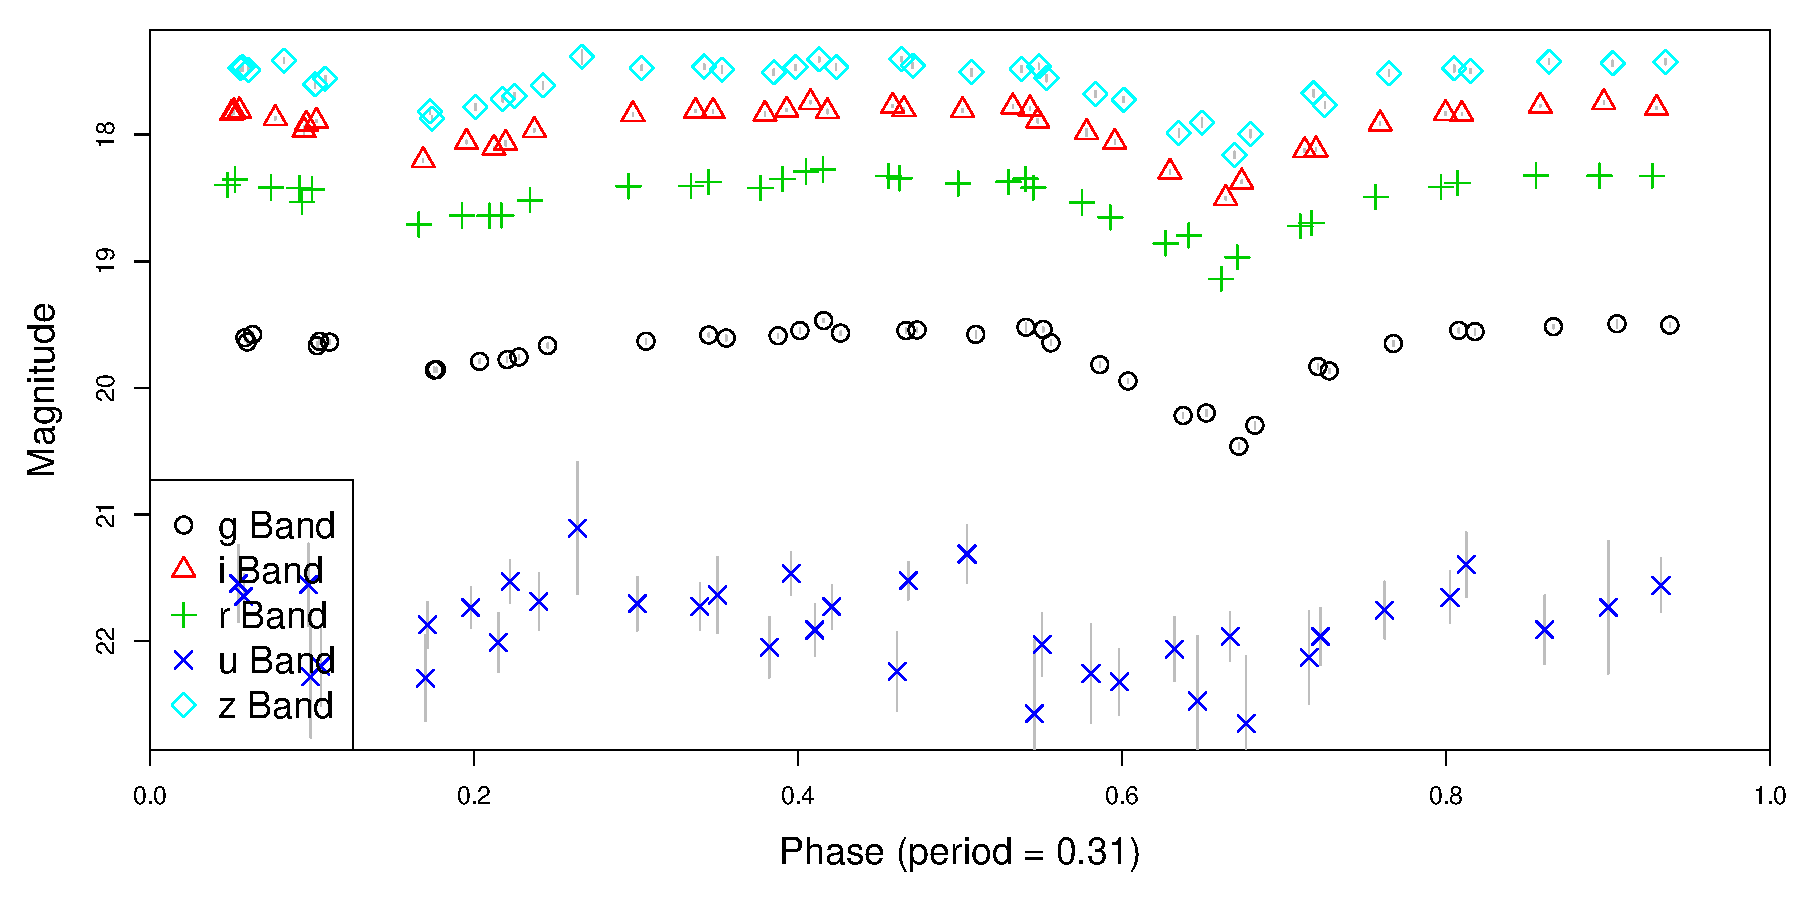
\includegraphics[scale=.15]{figs/folded_4183016.pdf}
\end{center}

\vspace{-.2in}

%% \begin{center}
%% RR Lyrae\\
%% 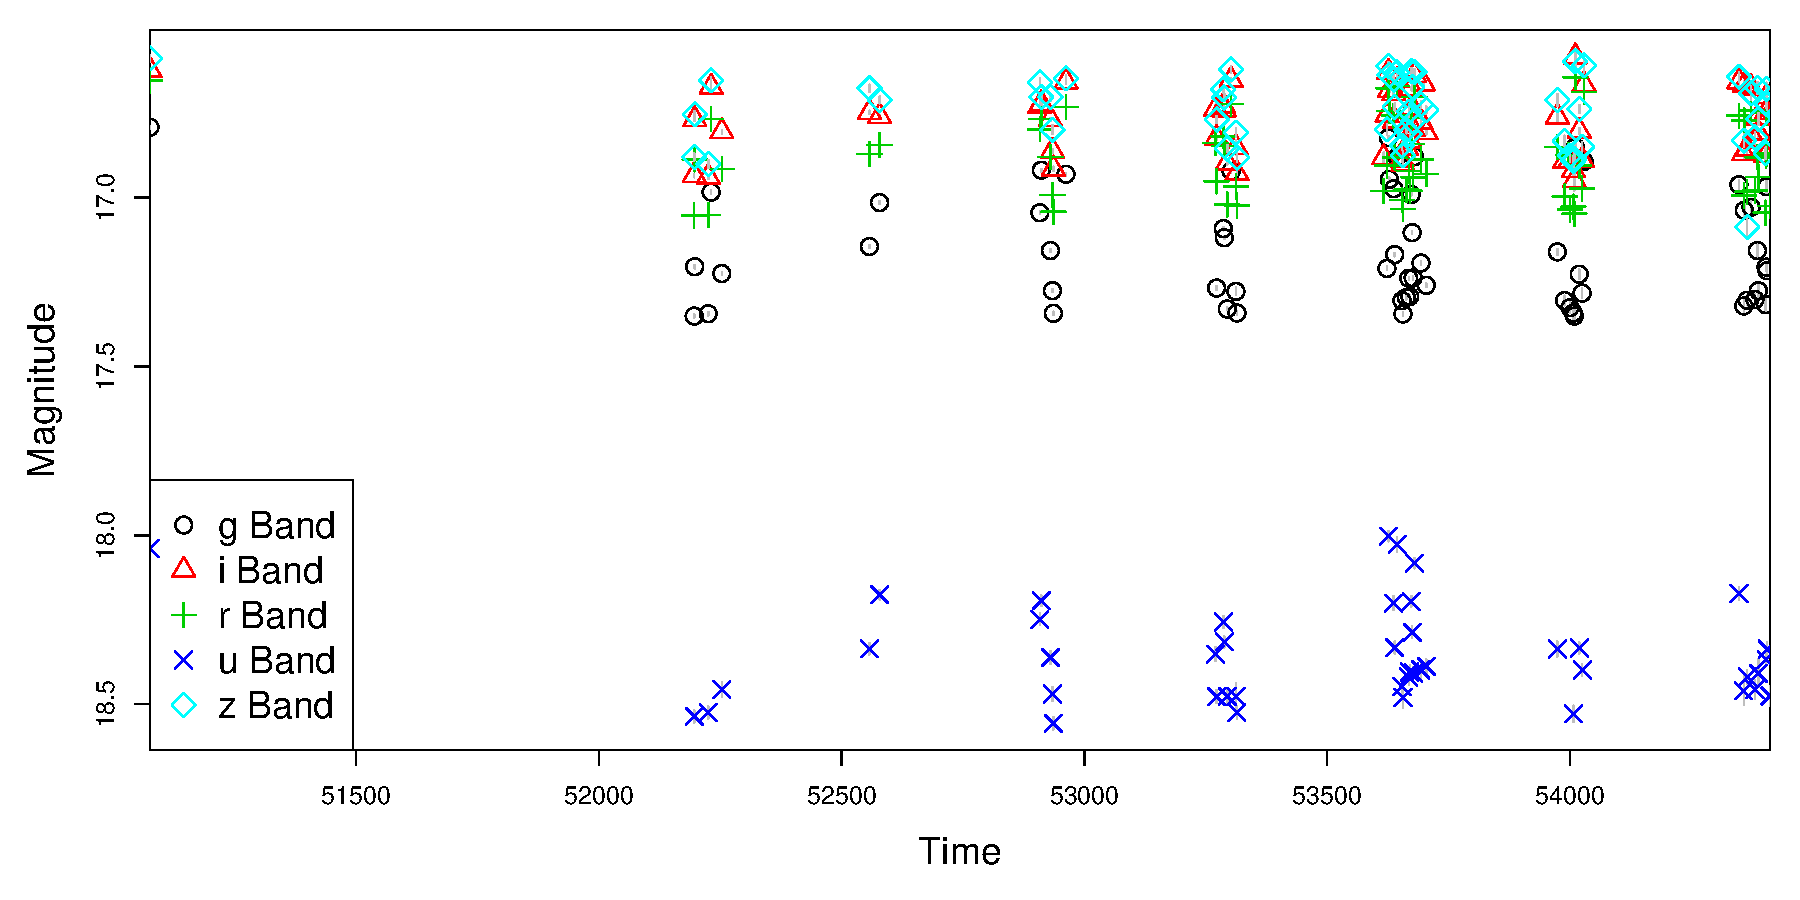
\includegraphics[scale=.15]{figs/unfolded_4099.pdf}
%% 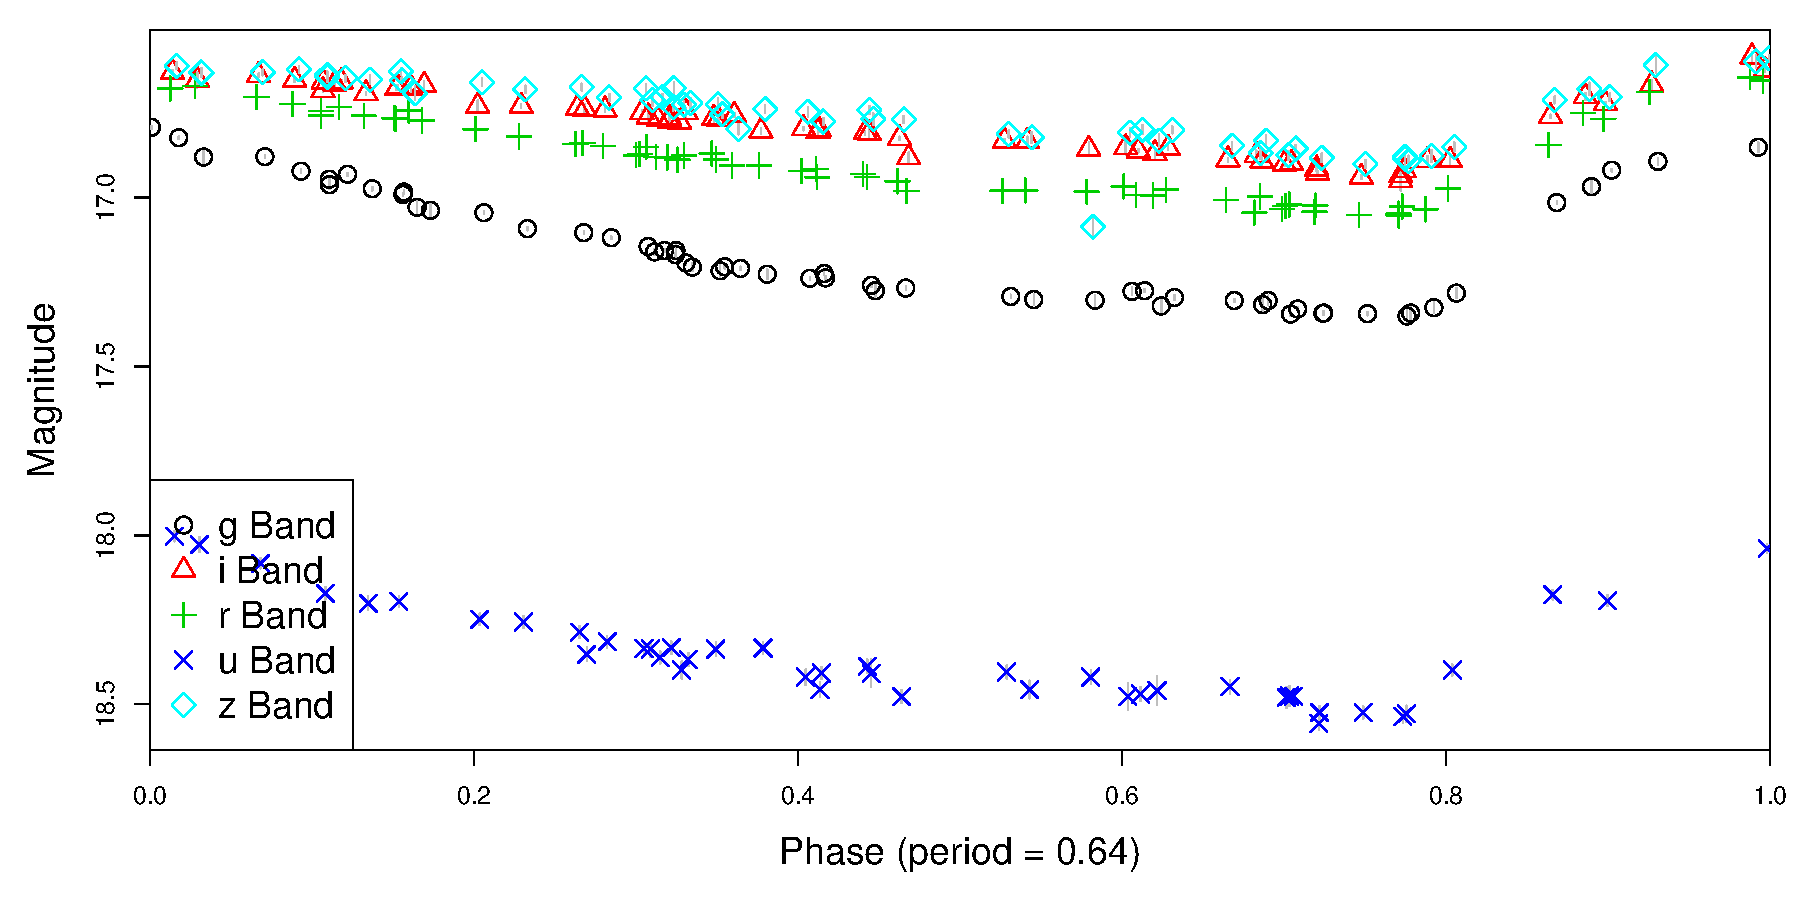
\includegraphics[scale=.15]{figs/folded_4099.pdf}
%% \end{center}


\begin{center}
Quasar\\
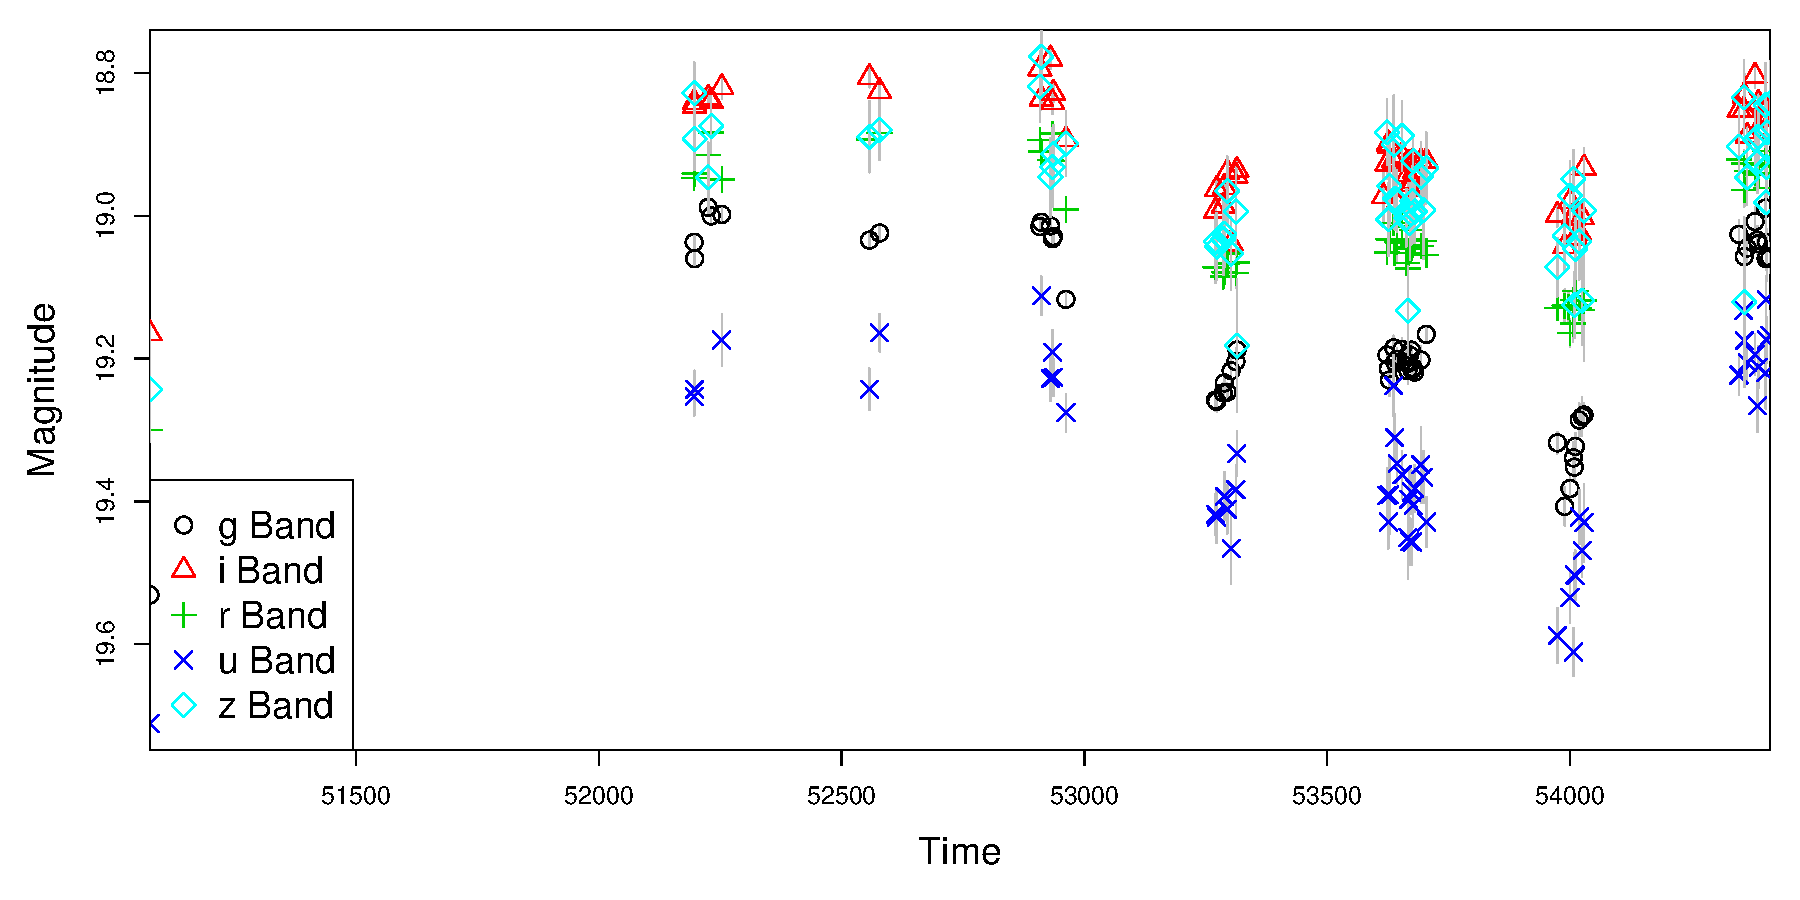
\includegraphics[scale=.15]{figs/unfolded_7904669.pdf}
\end{center}


\end{frame}


\begin{frame}{Variable Star Analysis Pipeline}
\begin{itemize}
\item Identify Variable Stars.
\item Estimate parameters for variables: period, amplitude, shape, etc.
\item Classify stars.
\item Do science: period luminosity relations, distance determination.
\end{itemize}
\end{frame}


%% \begin{frame}{Size of Variable Star Data Sets is Growing}
%% \begin{itemize}
%% \item \textit{Hipparcos} (1989--1993): 2712 
%% \item \textit{OGLE} (1992--present): 100,000s
%% \item \textit{DES} (ongoing): $\sim$ 10 million
%% \item \textit{LSST} (starting 2020): $\sim$ 1 billion

%% \vspace{.4in}

%% Data sets of varying quality:
%% \begin{center}
%% 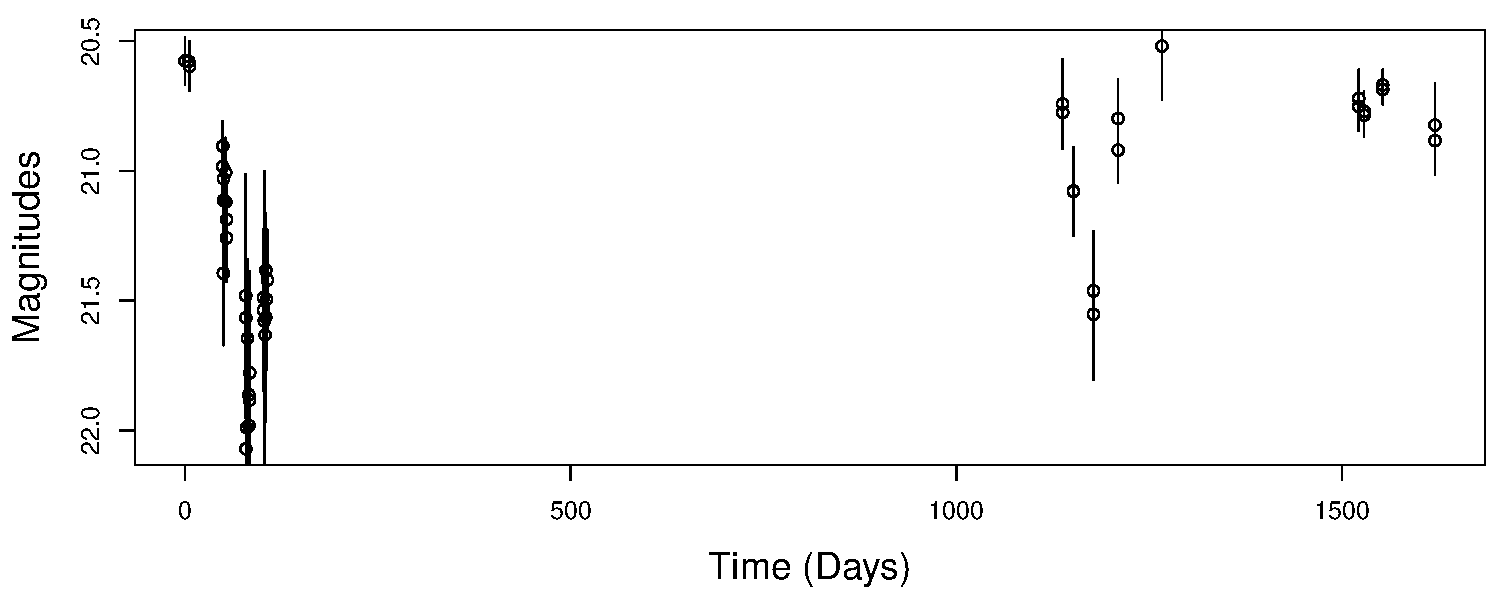
\includegraphics[scale=.3]{figs/m33_unfolded.pdf}
%% \end{center}


%% \end{itemize}

%% %\textbf{Dramatic Differences in Data Quality:}

%% \end{frame}



%%%%%%%%
%%%%%%%% TODO: discuss panstarrs / DES, performance of lomb scargle
%%%%%%%%

\section{Period Estimation Methods}



\begin{frame}{Sinusoid Based Models}

\textbf{Method:} Model light curve variation in each filter as sinusoid with $K$ harmonics. \cite{mondrik2015multiband,zechmeister2009generalised,lomb1976least,scargle1982studies,schwarzenberg1996fast}

\begin{equation*}
m_{jb} = \beta_b + \sum_{k=1}^K a_{bk}\sin(\omega t_{jb} + \phi_{bk}) + \epsilon_{jb}
\end{equation*}
where $\epsilon_{jb} \sim N(0,\sigma_{jb}^2)$.

\begin{itemize}
\item $(2K + 1)B + 1$ parameters. Pure sine $3B + 1$ parameters.
\item Maximum likelihood has closed form solution at fixed $\omega$
\begin{itemize}
\item Maximization strategy: Grid search on $\omega$.
\end{itemize}
\end{itemize}

\end{frame}


\begin{frame}{Example of Maximum Likelihood Fit with $K=2$}

\vspace{-.1in}

\begin{center}
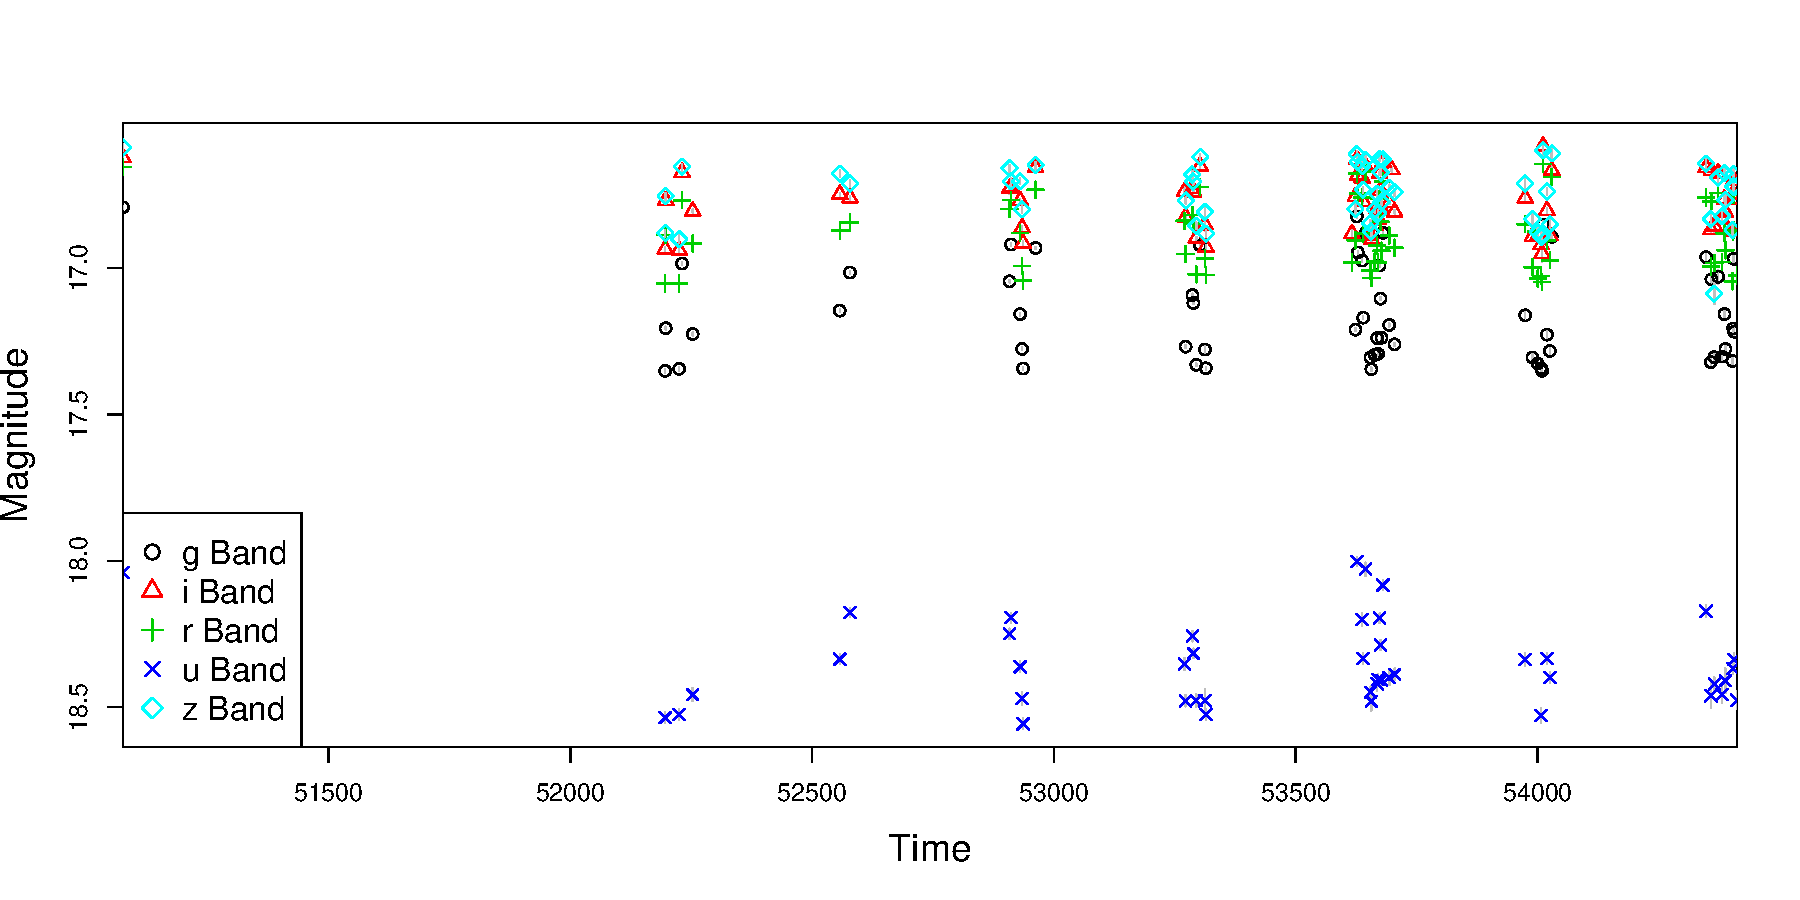
\includegraphics[scale=.25]{figs/rrlyrae_nomodel_fit.pdf}\\
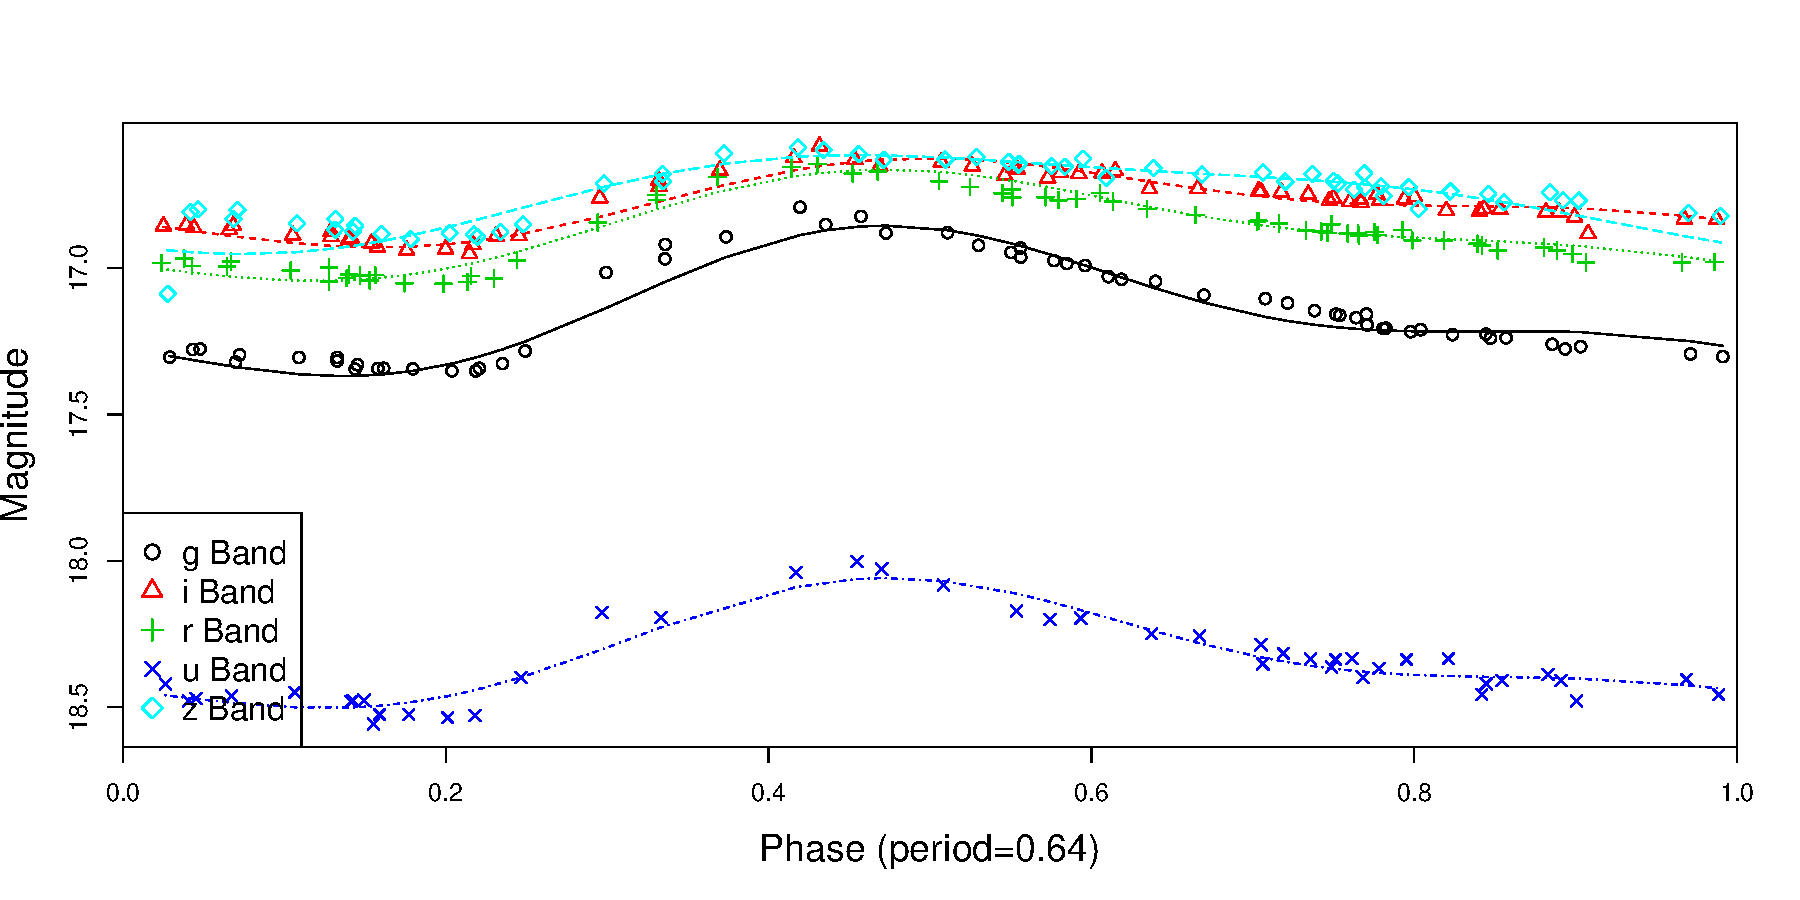
\includegraphics[scale=.25]{figs/rrlyrae_model_fit.pdf}\\
Total of $26$ parameters, model estimates period well.
\end{center}

\end{frame}

\begin{frame}{Output from Model Useful for Classification}

%%% TODO: make scatterplot of two features

\end{frame}


\begin{frame}{Dark Energy Survey (DES) and Pan--STARRS Data}

\begin{itemize}
\item some statistics on panstarrs and des lightcurves
\end{itemize}

Example of Pan--STARRS lightcurve.

\end{frame}








%%%%%%%%
%%%%%%%% TODO: introduce model, discuss fitting
%%%%%%%%


\section{Parsimonious Model for RR Lyrae Variables}

\begin{frame}{RR Lyrae Model}

\begin{equation*}
m_b(t) = \alpha + \beta_b + E[B-V]\delta_b + a\gamma_b(\omega t + \phi)
\end{equation*}

\underline{global parameters} common for all RR Lyrae are
\begin{align*}
\beta_b &=  \text{ magnitude off--set in band $b$ }\\
\delta_b &= \text{ attenuation caused by dust in band $b$ }\\
\gamma_b &= \text{ normalized shape of light curve in band $b$ }\\
\end{align*}
\underline{individual parameters} specific to each RR Lyrae are
\begin{align*}
\alpha &= \text{ mean brightness across all bands }\\
E[B-V] &= \text{ amount of dust }\\
a &= \text{ amplitude of variation }\\
\omega &= \text{ frequency of variation }\\
\phi &= \text{ phase }
\end{align*}

\end{frame}



\begin{frame}{$\gamma_b$ functions}

\begin{center}
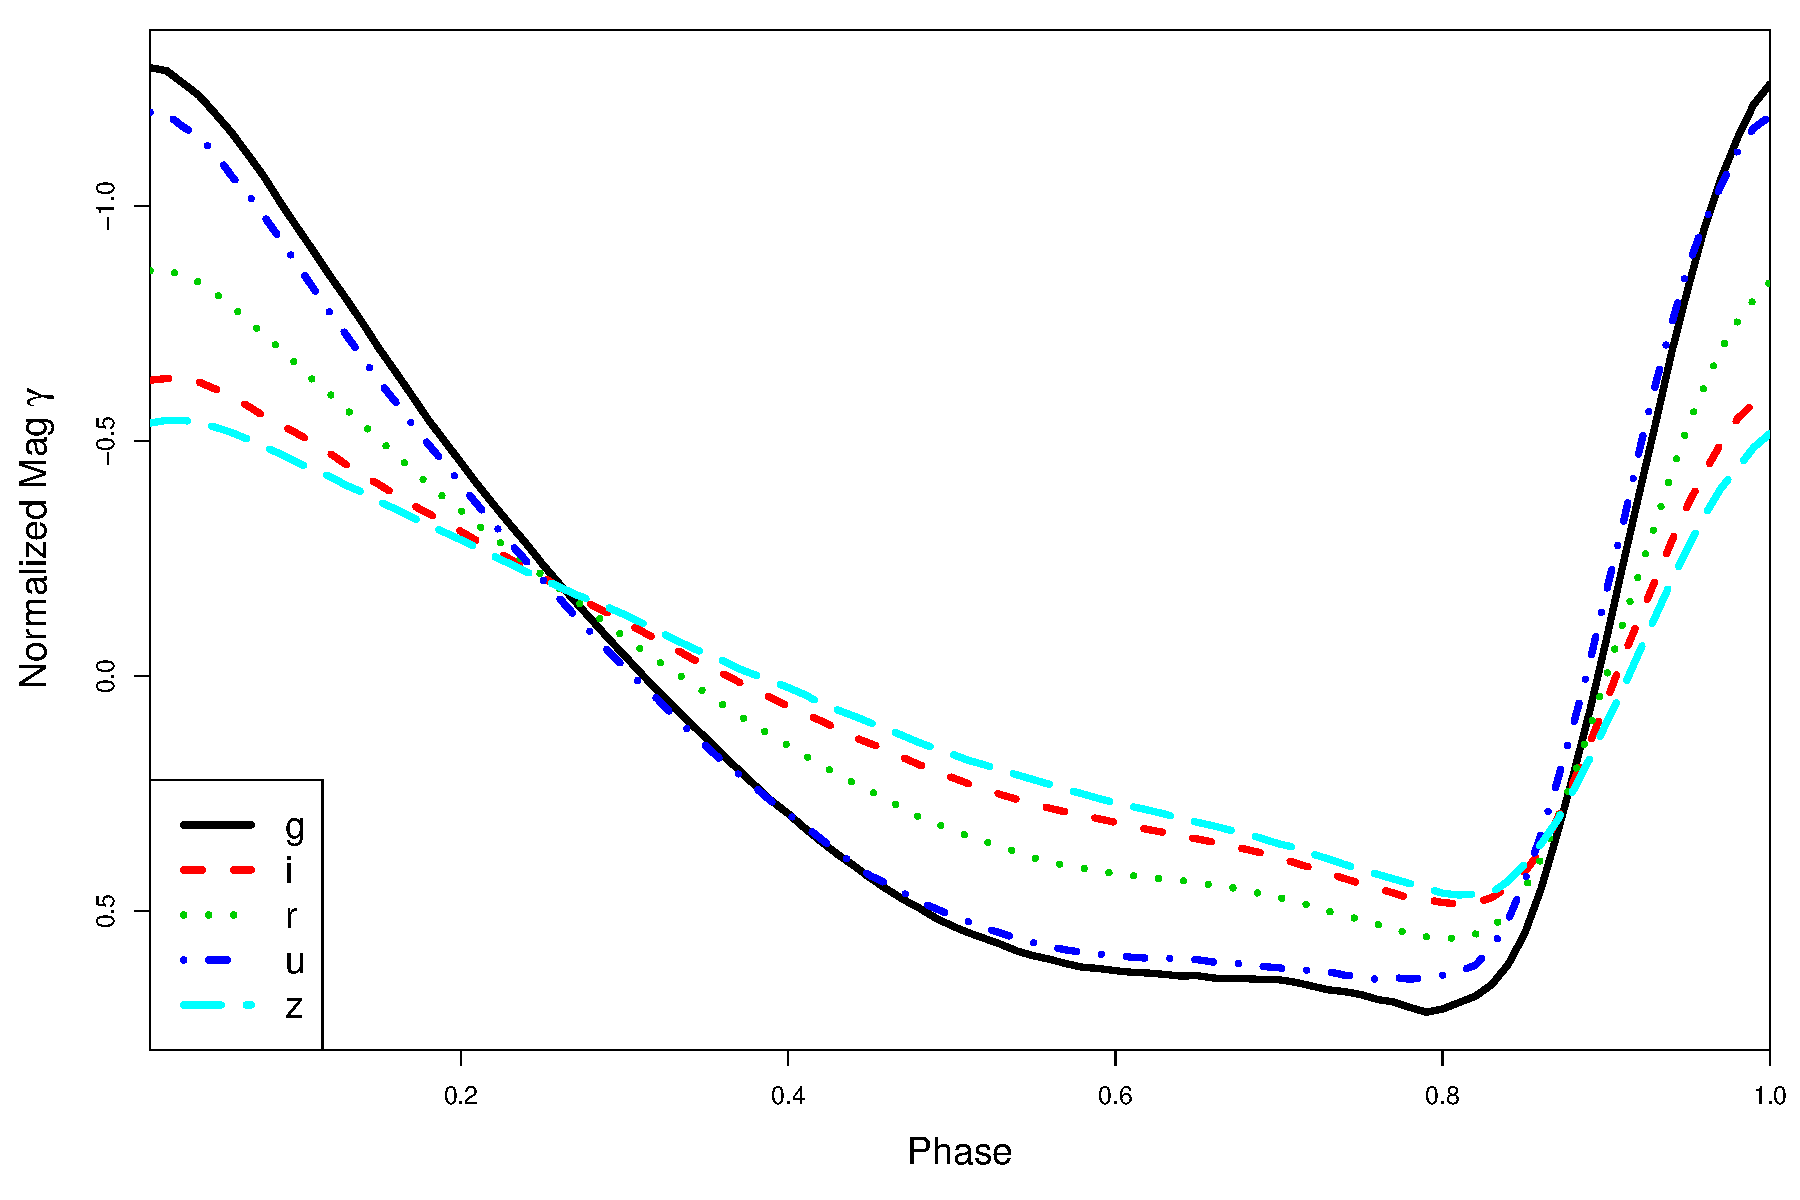
\includegraphics[scale=.3]{figs/templates.pdf}
\end{center}

\end{frame}


\begin{frame}{Parameter Estimation}

Define
\begin{align*}
&g(\omega,\alpha,E[B-V],a,\phi) \\
= &\sum_{b=1}^B \sum_{j=1}^{n_b}\left(\frac{m_{jb} - \beta_b - \alpha - E[B-V]\delta_b - a\gamma_b(\omega t_{jb} + \phi)}{\sigma_{bi}}\right)^2
\end{align*}

Estimate parameters with maximum likelihood ($\chi^2$ minimization):
\begin{itemize}
\item Likelihood is highly multimodal in $\omega$, grid search on frequency.
\item Model is linear in $\alpha$,$E[B-V]$, and $a$, closed form updates.
\item Newton--Raphson updates for $\phi$ parameter.
\end{itemize}

\end{frame}


\section{Results}

\begin{frame}{Simulation Results for Period Estimation}


\end{frame}


\begin{frame}{Simulation Results for Classification}


\end{frame}


\section{Conclusions and Future Work}

%% \begin{frame}{Folded Light Curve using Two Sinusoidal Models}
%% \begin{center}
%% 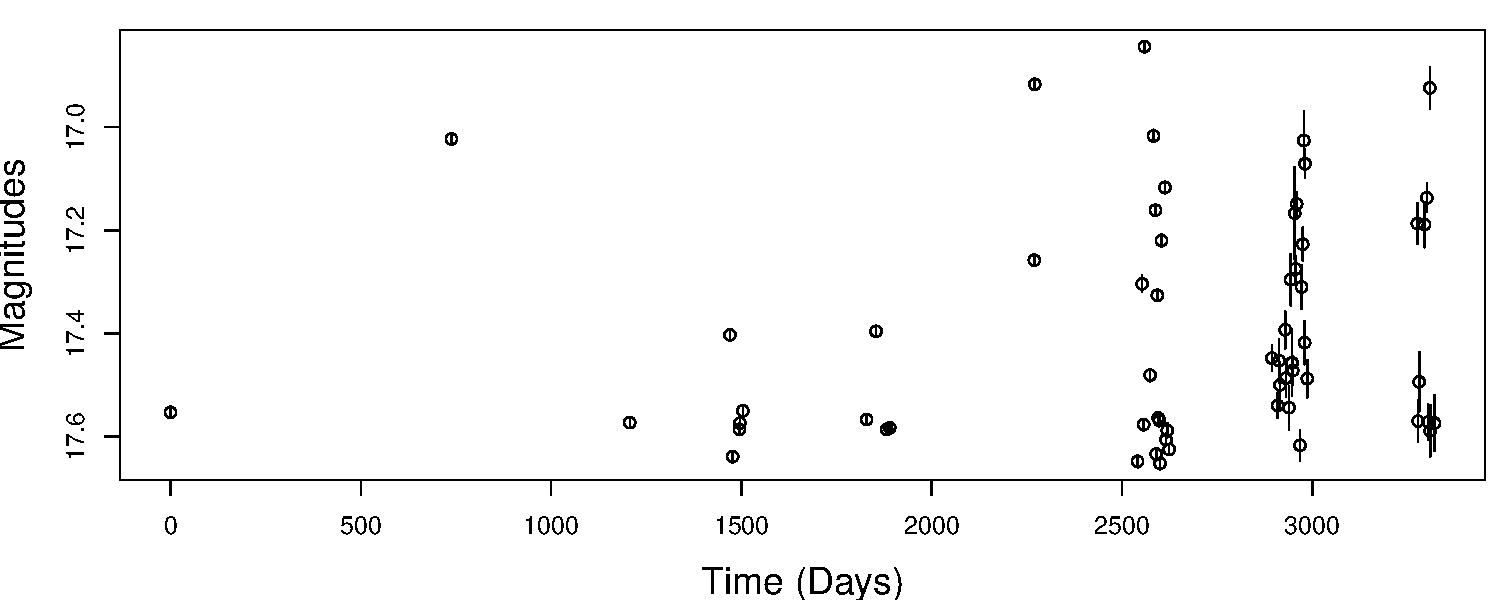
\includegraphics[scale=0.32]{figs/unfolded_single.pdf}\\
%% 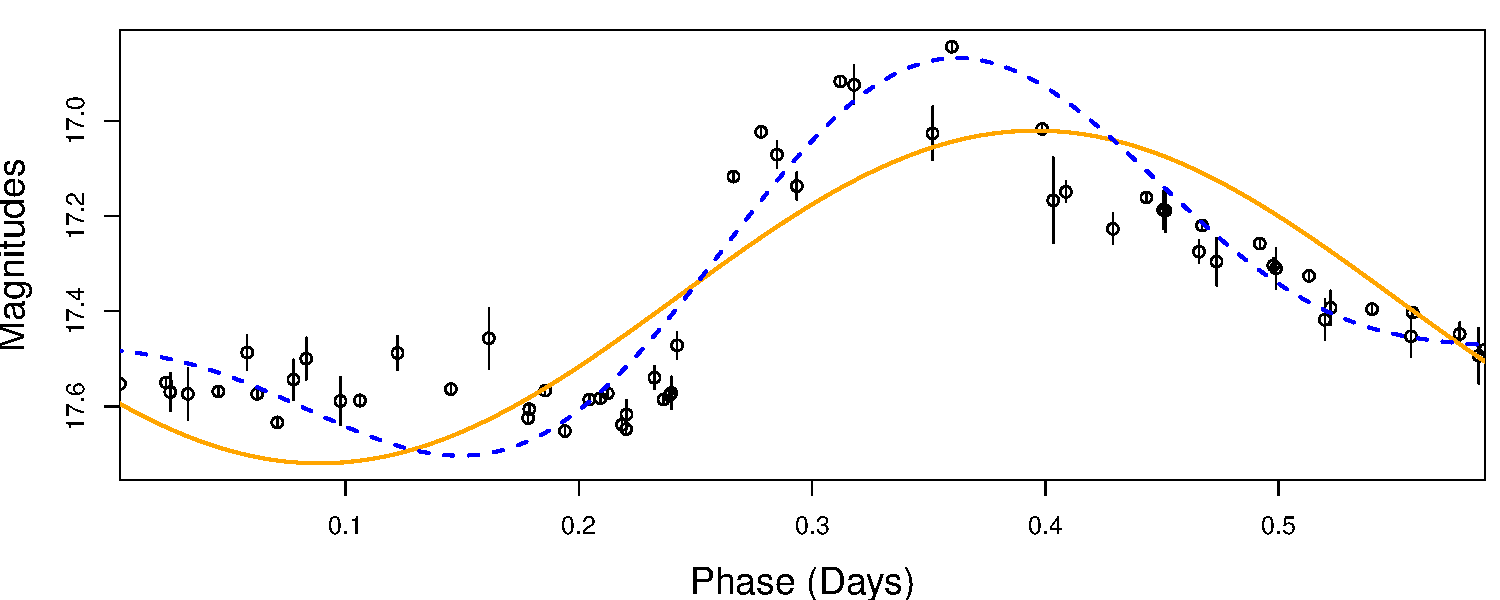
\includegraphics[scale=0.32]{figs/folded_single.pdf}
%% \end{center}
%% \end{frame}

%% \begin{frame}{Period Estimation for Variable Stars}
%% \textbf{Common Model:} 
%% \begin{equation*}
%% m_i = \beta_0 + \sum_{k=1}^K a_k \sin(t_i\omega k + \phi_k) + \epsilon_i
%% \end{equation*}
%% where $\epsilon_i \sim N(0,\sigma_i^2)$ {\tiny Zechmeister \cite{zechmeister2009generalised}, Schwarzenberg \cite{schwarzenberg1996fast}}

%% \vspace{.2in}

%% \textbf{Maximum likelihood estimator:}
%% \begin{equation*}
%% \widehat{\omega} = \argmin{\omega} \min_{\phi,a,\beta_0} \sum_{i=1}^n\left(\frac{m_i - \beta_0 - \sum_{k=1}^K a_k\sin(\omega t_ik + \phi_k)}{\sigma_i}\right)^2
%% \end{equation*}
%% \end{frame}



%% \begin{frame}{Question}
%% \begin{itemize}
%% \item Misspecified models are common and can be useful.
%% \item Heteroskedasticity in responses is common.
%% \item Typically we weight observations by inverse of variance.
%% \end{itemize}

%% \vspace{.3in}
%% \textbf{Question:} Is this weighting helpful when the model is misspecified?

%% \end{frame}


%% \begin{frame}{Example: Period Estimation for Variable Stars}
%% \begin{center}
%% 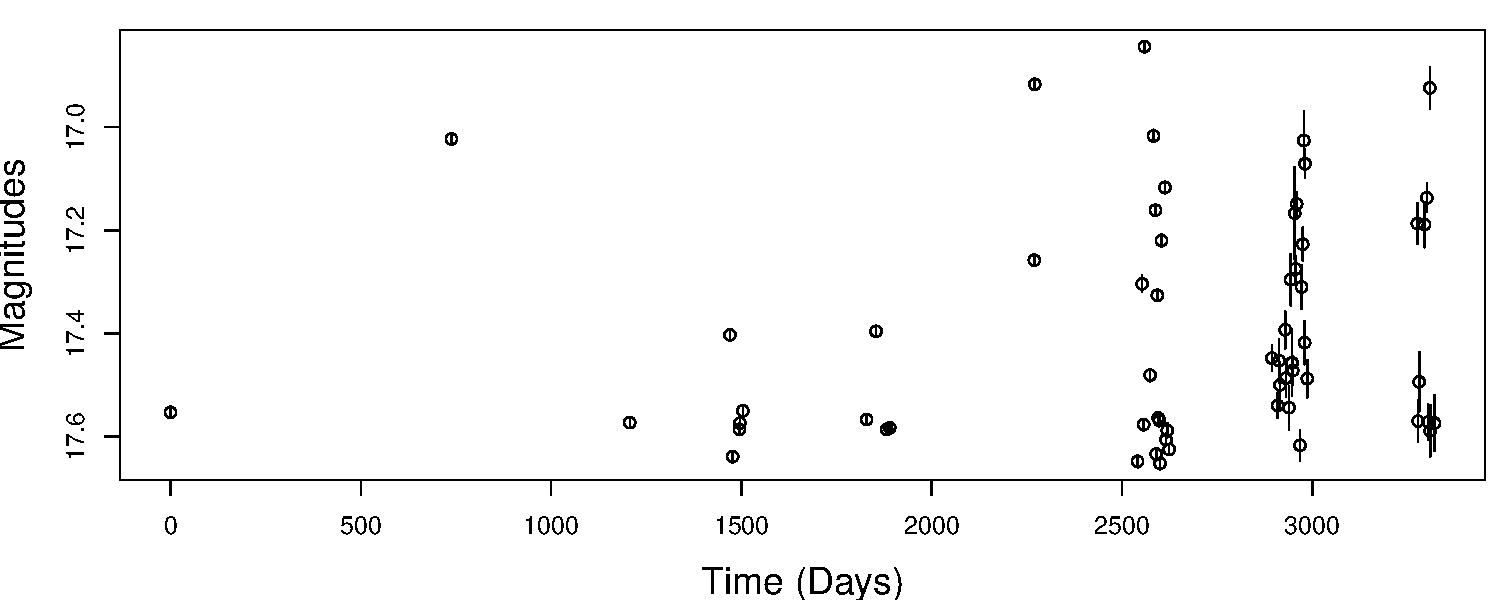
\includegraphics[scale=0.35]{figs/unfolded_single.pdf}
%% \end{center}
%% \textbf{Data:} $D = \{(t_i,m_i,\sigma_i)\}_{i=1}^n$
%% \begin{itemize}
%% \item magnitude $m_i$
%% \item observed at time $t_i$
%% \item with uncertainty $\sigma_i$
%% \end{itemize}
%% \vspace{.2in}
%% \textbf{Goal:} Estimate period, amplitude, etc. of star.
%% \end{frame}

%% \begin{frame}{hello}
%% \cite{zechmeister2009generalised}
%% \end{frame}



%% \begin{frame}{Simulate a sinusoidal light curve}
%%  % with $K=1$, $p = 2\pi / \omega = 1$, $a = 1$, $\beta_0 = 14$, $\beta_0 = 14$, $\sigma_i = 0.3$.

%% \begin{center}
%% \includegraphics[scale=.5]{code/figs/lc_sine.pdf}
%% \end{center}

%% \end{frame}

%% \begin{frame}{Correct Model}
%% \begin{center}
%% \includegraphics[scale=.5]{code/figs/sd1.pdf}
%% \end{center}
%% \end{frame}

%% \begin{frame}{Correct Model}
%% \begin{center}
%% \includegraphics[scale=.5]{code/figs/sd2.pdf}
%% \end{center}
%% \end{frame}

%% \begin{frame}{Correct Model: Weighted Fit}
%% \begin{center}
%% \includegraphics[scale=.5]{code/figs/sd3.pdf}
%% \end{center}
%% \end{frame}

%% \begin{frame}{Correct Model: Unweighted Fit}
%% \begin{center}
%% \includegraphics[scale=.5]{code/figs/sine_unweight.pdf}
%% \end{center}
%% \end{frame}


%% \begin{frame}{Correct Model}
%% \begin{center}
%% \includegraphics[scale=.5]{code/figs/sd5.pdf}
%% \end{center}
%% \end{frame}



%% \begin{frame}{Summary}
%% \begin{itemize}
%% \item The fitted curve (orange line) is close to observations with small  error (small $\sigma_i$).
%% \item This is good \textbf{when the actual light curve variation is sinusoidal.}
%% \end{itemize}

%% \vspace{.2in}
%% \textbf{Question:} What happens for misspecified models (light curves that are not actually sinusoids)?

%% \end{frame}


%% \begin{frame}{Simulate negative sawtooth (RR Lyrae like shape)}
%%  % with $K=1$, $p = 2\pi / \omega = 1$, $a = 1$, $\beta_0 = 14$, $\beta_0 = 14$, $\sigma_i = 0.3$.

%% \begin{center}
%% \includegraphics[scale=.5]{code/figs/lc_sawtooth.pdf}
%% \end{center}

%% \end{frame}



%% \begin{frame}{Misspecified Model -- Weighted Fit}
%% \begin{center}
%% \includegraphics[scale=.5]{code/figs/sd1wrong.pdf}
%% \end{center}
%% \end{frame}

%% \begin{frame}{Misspecified Model -- Weighted Fit}
%% \begin{center}
%% \includegraphics[scale=.5]{code/figs/sd2wrong.pdf}
%% \end{center}
%% \end{frame}

%% \begin{frame}{Misspecified Model -- Weighted Fit}
%% \begin{center}
%% \includegraphics[scale=.5]{code/figs/sd3wrong.pdf}
%% \end{center}
%% \end{frame}

%% \begin{frame}{Misspecified Model -- Unweighted Fit}
%% \begin{center}
%% \includegraphics[scale=.5]{code/figs/sd_unweight.pdf}
%% \end{center}
%% \end{frame}







%% \section{Period Estimation and Classification for M33 Miras}

%% \begin{frame}{Collaboration}
%% %% astronomers
%%   \begin{textblock*}{12cm}(0cm,1cm) % {block width} (coords)
%% \begin{center}
%% \textbf{Astronomy}
%% \end{center}
%% \end{textblock*}
%%   \begin{textblock*}{3cm}(3.5cm,2cm) % {block width} (coords)
%% 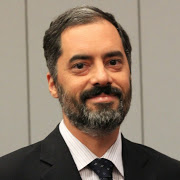
\includegraphics[width=\w,height=\h]{figs/Macri.jpg}\\
%% Lucas Macri
%% \end{textblock*}
%%   \begin{textblock*}{3cm}(7cm,2cm) % {block width} (coords)
%% \includegraphics[width=\w,height=\h]{figs/yuan.jpg}\\
%% Wenlong Yuan
%% \end{textblock*}


%% %% statisticians
%%   \begin{textblock*}{12cm}(0cm,5.1cm) % {block width} (coords)
%% \begin{center}
%% \textbf{Statistics}
%% \end{center}
%% \end{textblock*}

%%   \begin{textblock*}{3cm}(1.5cm,6.1cm) % {block width} (coords)
%% \includegraphics[width=\w,height=\h]{figs/he.jpg}\\
%% Shiyuan He
%% \end{textblock*}


%%   \begin{textblock*}{3cm}(5cm,6.1cm) % {block width} (coords)
%% \includegraphics[width=\w,height=\h]{figs/Huang2.jpg}\\
%% Jianhua Huang
%% \end{textblock*}

%%   \begin{textblock*}{3cm}(8.5cm,6.1cm) % {block width} (coords)
%% \includegraphics[width=\w,height=\h]{figs/long2.jpg}\\
%% James Long
%% \end{textblock*}
%% \end{frame}


%% \begin{frame}{Period Luminosity Relation for Miras in the LMC}


%% %% \begin{textblock*}{3cm}(8cm,1.5cm) % {block width} (coords)
%% %% \includegraphics[scale=.25]{figs/lmc2.jpg}\\
%% %% \end{textblock*}

%% \begin{textblock*}{3cm}(1cm,1.5cm) % {block width} (coords)
%% \includegraphics[scale=.25]{figs/lmc2.jpg}
%% \end{textblock*}




%% \begin{textblock*}{3cm}(6cm,1.5cm) % {block width} (coords)
%% \includegraphics[scale=.22]{figs/period_luminosity_miras.pdf}
%% \end{textblock*}



%% \begin{textblock*}{3cm}(3cm,5.5cm) % {block width} (coords)
%% \includegraphics[scale=.25]{figs/mira1_unfolded.pdf}\\
%% \end{textblock*}


%% \end{frame}


%% \begin{frame}{PL Relation for Miras in M33}

%% \begin{textblock*}{3cm}(8cm,2.5cm) % {block width} (coords)
%% 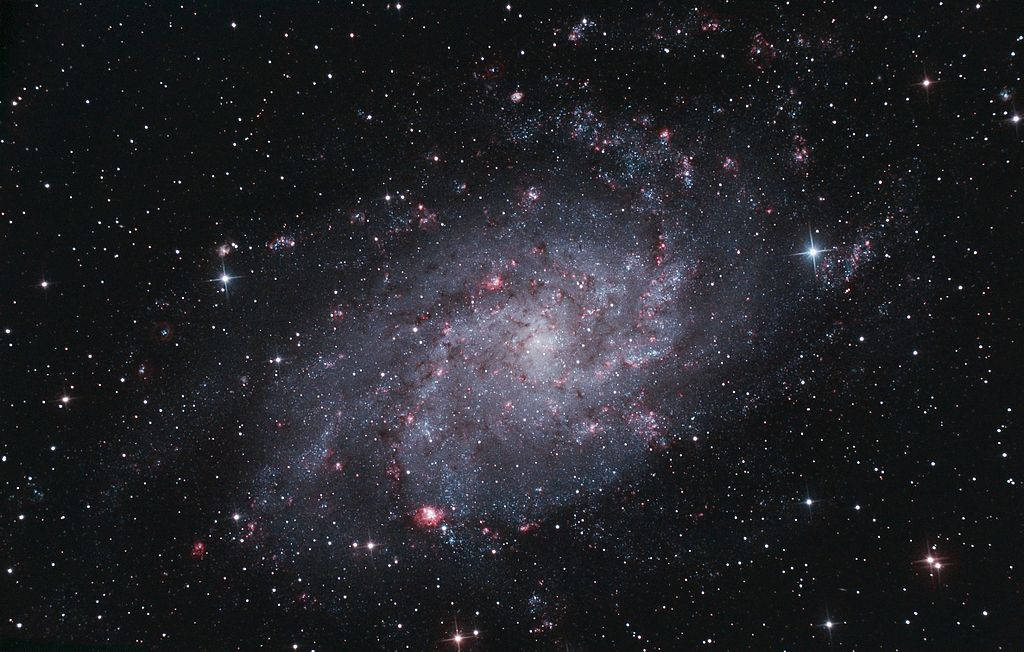
\includegraphics[scale=.1]{figs/m33.jpg}
%% \end{textblock*}




%% \textbf{Estimating PL Relation requires:}



%% \begin{itemize}
%% \item Estimating periods and luminosities accurately.
%% \item Classifying stars.
%% \end{itemize}


%% \vspace{.3in}

%% \textbf{Challenging case:}
%% \begin{center}
%% 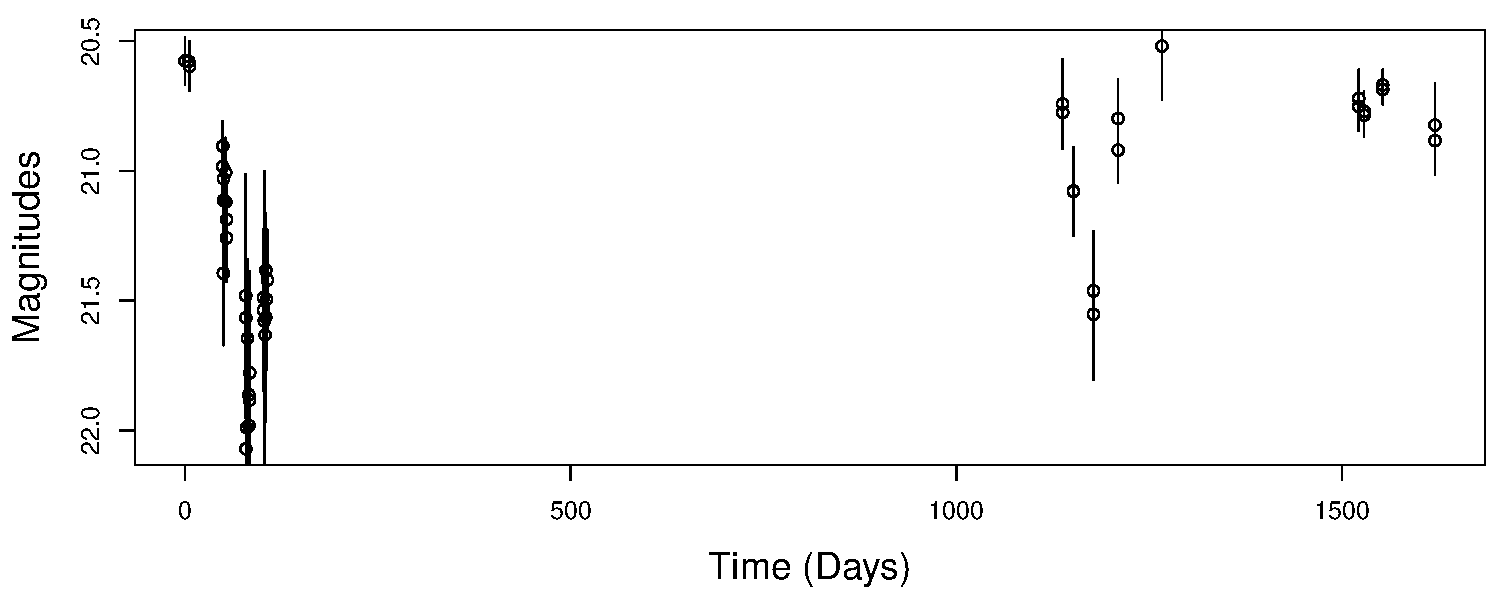
\includegraphics[scale=.4]{figs/m33_unfolded.pdf}
%% \end{center}

%% \end{frame}


%% \begin{frame}{Sinusoid Fit to LMC Mira}

%% \begin{center}
%% \includegraphics[scale=.3]{figs/mira4_unfolded_fit.pdf}\\
%% \includegraphics[scale=.3]{figs/mira4_folded_fit.pdf}
%% \end{center}

%% \end{frame}


%% \begin{frame}{Fit to M33 Mira}

%% \begin{center}
%% \includegraphics[scale=.3]{figs/m33_unfolded_fit.pdf}\\
%% \includegraphics[scale=.3]{figs/m33_folded_fit.pdf}
%% \end{center}

%% \vspace{.05in}

%% Improve sinusoidal model to accurately estimate periods with M33.

%% \end{frame}


%% \begin{frame}{Gaussian Process Fit to OGLE Mira}
%% \begin{center}
%% \includegraphics[scale=.4]{figs/mira3_GP.pdf}
%% \end{center}

%% %% \begin{align*}
%% %% \widehat{\theta}_{1} &= 1.4\\
%% %% \widehat{\beta}_{1} &= 1.4\\
%% %% \widehat{\beta}_{2} &= 2.4\\
%% %% \end{align*}
%% \end{frame}


%% \begin{frame}{Bayes Factors for Separating Different Classes}
%% \begin{center}
%% \includegraphics[scale=0.2]{figs/bayes_factor.png}
%% \end{center}
%% \end{frame}


\begin{frame}[allowframebreaks]{Bibliography}
%  \def\newblock{\hskip .11em plus .33em minus .07em}
%  \nocite{*}
%\nocite{*}
\bibliographystyle{plain} 
  \tiny{
  \bibliography{refs}}
\end{frame}

\end{document}


